The public opinion is one of the key factors for the success of a movie. To analyze and identify public opinion, we developed a sentiment analysis tool that, using tweets and comments from YouTube trailers, provides the following: \textit{i} The general public opinion about a movie; \textit{ii} The identification of the main topics on the evaluated texts; and \textit{iii} A ``recommendation text'' for the movie, based on the most relevant mentioned words. Next subsections describe all phases of the development to reach the proposed goal.

\subsection{Methodology}

Figure~\ref{fig:approach} presents our research methodology 
%, which is presented in , and 
which is divided into four steps. The first one consists of collecting data from social media. On this step, we gathered data from both YouTube and Twitter, using the tools described in Subsection~\ref{sec:datasetCollection}. 

After the data gathering step, we preprocess the collected data. During this second step, we remove texts' links, distribute the data in a temporal series, and tokenize the text. We did not remove the stopwords because they are used by Vader Lexicon uses them on the evaluation process.
% I: o que é a saída desta segunda etapa? O que é gerado? Também acho que a última frase do parágrafo acima deve ser alterada para: "We did not remove the stopwords because they are used by Vader Lexicon on the evaluation process.". Do jeito como está agora "use" aparece duas vezes na frase.

On the third step, we used Vader to perform Sentiment Analysis on our texts. This analysis provides us the sentiment scores and compound values (see section \ref{vader}) for the tweets and comments collected. The texts are then split into several files, according to their polarity. 
% I: não daria para complementar acima? Se eu entendi corretamentamente, no final do parágrafo acima poderia ter algo: Thus, we generate five files with the following content: (1) very positive; (2) positive; (3) neutral; (4) negative; and (5) very negative tweets and YouTube comments.
% Seria isto?

The fourth step of our study is the Data Analysis. On this step, we calculate the TF-IDF (see section \ref{TFID}) statistics using the files generated on the previous step. These statistics provided us information about the most frequent and relevant terms on the documents. 
% I: o que seria "documents" acima? É preciso especificar (já na metodologia) o que é gerado em cada etapa e usar sempre a mesma terminologia.

In this step, we use the TF-IDF features to evaluate how important a certain term/word is in a given document~\cite{Dipanjan:2016}. The results obtained by the sentiment analysis with Vader, were divided into files, according to the polarity defined by the lexicon in each text, and then the TF-IDF was applied. Therefore, we will have the most used terms in negative and positive texts. From the most used terms found in the texts, we proceed to the identification the lexical category in which the words are assigned based on their syntactic context and role, called POS (Part-of-Speech) Tagging. Using NLTK Library\footnote{https://www.nltk.org/}, which generates outputs specific tags for certain word, we could find: \textit{Adjectives, Nouns, Adverbs, Coordination Conjunction, Verbs, Preposition and etc}, as showed in Listing \ref{tfidf}.

In this step, we also generate 3 kinds of visualization graphics one for each social media we chose. The first one is a bar chart that displays the overall number of comments obtained for the selected movies on both social media. Each bar presented on this visualization represents one sentiment polarity (very positive, positive, negative and very negative). We opted to display the social media side by side to simplify users' comparison. 

The second visualization provides word clouds, showing the most used words for negative and positive sentiment polarity. For this visualization, we chose to use only verbs, noun, and adjective grammar types, because, for this case, we believe that those are the most significant ones. Like the previous visualization, 2 word clouds are generated for each social media, one for the most used words in negative comments, and another one for the most used words in positive comments. 

On the third visualization, a heatmap is presented. This visualization presents the top 10 most used adjectives in comments for the movie's characters. For this visualization, we present only characters for whom we were able to find mentions in the analyzed text. This visualization is split by sentiment polarity (positive and negative) and by social media (Twitter and YouTube). These visualizations can be seen in Figures ~\ref{fig:TotalOfInteractions},~\ref{fig:wordcloudsAquaman},~\ref{fig:wordcloudsCaptain},~\ref{fig:wordcloudsAvengers},~\ref{fig:AquamanCapitaHeatMap} and \ref{fig:VingadoresHeatMap}

\begin{figure*}[t!]
\begin{center}
% \fbox{\rule{0pt}{2in} \rule{.9\linewidth}{0pt}}
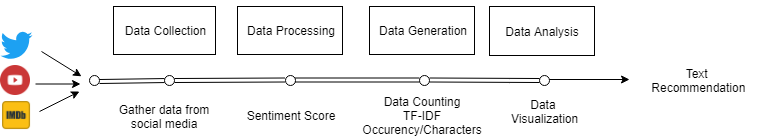
\includegraphics[width=0.8\linewidth]{img/Lexicon.png}
\end{center}
   \caption{Proposed approach overview: from data gathering to text recommendation.}
\label{fig:approach}
\end{figure*}


%\newcommand*\latin[1]{\textit{}}

\subsection{Dataset Extraction}
\label{sec:datasetCollection}

For the context of movie reviews, we decided to analyze data from Twitter and YouTube comments about trailers. Twitter is used to quickly express opinions, and YouTube is a social media widely adopted to display movie trailers. We developed and used Python scripts to gather the desired data from the officials APIs of these social media. 

% I: abaixo não seria melhor que dizer que usaram hashtags ao invés de keywords? Achei estranho dizer que usaram hashtags ao invés da web page oficial... Se a ideia é coletar opinião das pessoas, também não faz sentido coletar dados do perfil do studio... Como aqui é uma seção mais "genérica", que descreve a abordagem, sugiro alterar a última frase para: Thus for each movie, it is possible to use a different set of hashtags to be collected. Ainda, não sei se é usual dizer "Comments on Twitter" ou simplesmente se usa "Tweets". Acho melhor começar com: Tweets usually contain hashtags to indicate their subject.
%like youtube
Twitter usually contain hashtags to indicate the subject of its text. For this reason, we chose to collect data through the use of hashtags instead of using keywords. We believe that the use of hashtags would provide a higher number of information and better quality data. The Twitter API implements features that allow the user to provide a hashtag list with the subjects to be collected. Thus for each movie, we selected a different set of hashtags to be collected. 

The YouTube comments were collected from the Studios' officials channels. We collected data from all the officials' trailers released for a movie. In this analysis, we did not collect data from teasers. We only collect data from the top level of comments on YouTube. This decision was made because on the lower levels, the comments, generally, serve as an answer to previous comments and are not properly related to the movie. 

% I: estou em dúvida se o parágrafo abaixo não deveria ser o segundo parágrafo desta subseção. A ideia seria primeiro dizer como funcionam os scripts e depois explicar como foram feitas as coletas no contexto deste trabalho. Por exemplo, no Twitter foram usadas hashtags, e para o YouTube foram escolhidos os trailers oficiais dos studios. Trouxe para cá um texto que estava mais abaixo, e deixei os próximos dois parágrafos só com a descrição do que é coletado de cada rede social. Vejam se concordam com as alterações.
Both of our scripts are straight forward to use. The Twitter script just requires a list of hashtags to be collected and the YouTube script only requires the video ID. The video ID is easily spotted on its web address. The data collected from both scripts are stored on JSON files. The scripts used for data collection, along with a detailed description of how to use them, can be found on https://github.com/DAVINTLAB/TweetProcessing..

% I: O parágrafo abaixo, vejam se concordam, original em comentário.
From Twitter, we collected data such as: \textit{username}, an internal user identification; \textit{lang}, the language in which the tweet was written; \textit{screen\_name}, user's name showed on screen; \textit{text}, the tweet written text; \textit{created\_at}, the date when the tweet was created; \textit{userid}, internal user identification; \textit{timezone}, the time zone in which the tweet was written; \textit{retweet\_count}, the number of times the tweet was re-posted; \textit{ID}, internal tweet identification; \textit{favorite\_count}, number of times other users liked this tweet.
% User Name, an internal user identification (username); Language, the language in which Twitter was written (lang); Screen Name, user's name showed on screen (screen\_name); Text, the tweet written text (text); Created at, the date when the tweet was created (created\_at); User id, internal user identification (userid); Time Zone, the timezone in which Twitter was written; Retweet count, the number of times this tweet was re-posted (retweet\_count); ID, internal tweet identification; (id), Favorite count, number of times other users liked this tweet (favorite\_count).

From YouTube script, we collected the following data: \textit{publishedAt}, the date when the comment was posted; \textit{textOriginal}, the original comment text; \textit{likeCount}, the number of times another users liked the comment; and \textit{authorDisplayName}, the author name that is displayed on the screen. 
% From YouTube script, we collected the following data: Published at, the date when the comment was posted (publishedAt); Original Text, the comment text (textOriginal); Like Count, the number of times another user's liked this comment (likeCount); and Author Display Name, the authors name displayed on the screen (authorDisplayName).  

% I: alterei abaixo. Vejam se concordam. Original em comentário.
Besides the Twitter and YouTube scripts, we also developed a third script for the IMDB site. The main goal of this script is to provide a list of all the characters of a movie. Since the IMDB website does not provide an official API for this purpose, we used the free IMDBPY API\footnote{https://imdbpy.sourceforge.io/}.
%Since the IMDB website does not provide an official API for this purpose, we used IMDBPY API. This API is free to use and it is available on https://imdbpy.sourceforge.io/.



\subsection{Unsupervised Lexicon-Based Sentiment Analysis}

Sentiment analysis, also known as opinion mining, is a sub-field of Natural Language Processing (NLP)\cite{Indurkhya:2010}. The main purpose of Sentiment Analysis is to identify and extract impressions/opinions from a particular text~\cite{vader}. Still many researches are going on to find out better alternatives due to its importance in this scenario\cite{DEVIKA201644}. 

Machine Learning is a widely used approach, and work by training an algorithm with a training data set, before applying it to the real data set\cite{DEVIKA201644}. This technique, first train the algorithm with some initials inputs, with known outputs, so that later it can work with new data\cite{He:2012}.

Lexicon based techniques work on an assumption that the collective polarity of a sentence or documents is the sum of polarities of the individual phrases or words\cite{DEVIKA201644}. The term polarity lexicon is used to refer to a dictionary or vocabulary with the indications of positive and negative words with an associated score~\cite{Dipanjan:2016}. The difference between both approaches, is that the lexicon based doesn't need labeled data for testing. 

Classification techniques are based on word position, surrounding words, context analysis, part-of-speech, phrases, and others. Various lexicons may be used for this analysis. Examples are: AFINN Lexicon~\cite{afinn}\cite{anew}, Bing Liu's Lexicon~\cite{Jinda}, MPQA subjectivity Lexicon~\cite{Wilson}, SentiWordNet~\cite{esuli-sentiwordnet}\cite{baccianella-sentiwordnet}, Vader Lexicon~\cite{vader}, Pattern Lexicon~\cite{pattern}. 

% Sentiment analysis, also known as opinion mining, is a sub-field of Natural Language Processing (NLP) \cite{Indurkhya:2010}. %SO: aqui seria legal uma ref tb
% % I: também acho que precisa referência acima, talvez para algum livro ou paper sobre "Sentiment analysis", que não seja o Vader.
% The main purpose of Sentiment Analysis is to identify and extract impressions/opinions from a particular text~\cite{vader}. Still many researches are going on to find out better alternatives due to its importance in this scenario\cite{DEVIKA201644}. 

% Machine Learning is a widely used approach, and work by training an algorithm with a training data set, before applying it to the real data set\cite{DEVIKA201644}. This technique, first train the algorithm with some initials inputs, with known outputs, so that later it can work with new data\cite{He:2012}.

%SO: porque ???
%and so we needed to develop mechanisms to overcome this difficulty. To overwhelm the annotated data problem, we resorted to unsupervised learning techniques. Those techniques use ontologies, databases, and lexicons with detailed information about the specific activity.
%SO:acima "tthose techniques"? citar refs...

% In those situations, we need discover another ways to classified this data. Unsupervised Techniques for predicting the sentiment by using ontologies, databases, and lexicons that have detailed information to specific activity are recommend options. 
%Sentimental analysis, also known as opinion mining, is a sub-field of Natural Language Processing (NLP).It's main goal is to identify and extract opinions from a particular text \cite{vader}. There are many approach's to apply sentiment analysis in texts, but when we hadn't labeled training data to learn patterns, that can be a issue. In those situations, we need discover another ways to classified this data. Unsupervised Techniques for predicting the sentiment by using ontologies, databases, and lexicons that have detailed information to specific activity are recommend options. 

% Isabel: colocar referência para paper ou livro que tenha a definiçao de lexicon.
% Lexicon based techniques 
% The term polarity lexicon is used to refer to a dictionary or vocabulary with the indications of positive and negative words with an associated score~\cite{Dipanjan:2016}.  Classification techniques are based on word position, surrounding words, context analysis, part-of-speech, phrases, and others. Various lexicons may be used for this analysis. Examples are: AFINN Lexicon~\cite{afinn}\cite{anew}, Bing Liu's Lexicon~\cite{Jinda}, MPQA subjectivity Lexicon~\cite{Wilson}, SentiWordNet~\cite{esuli-sentiwordnet}\cite{baccianella-sentiwordnet}, Vader Lexicon~\cite{vader}, Pattern Lexicon~\cite{pattern}. In the next section, we discuss the Vader Lexicon, which is used in our research. %SO: acima incluir refs please...

% Isabel: particularmente, acho que o vader poderia estar nesta seção, não precisaria ser uma seção separada. Acho que a seção III no momento está com muitas subseções.

%As mentioned, a lexicon is a dictionary or vocabulary, that have a list of positive and negative polar words with some score associate, and using some techniques like the position of words, surrounding words, context, part-of-speech, phrases and etc \cite{Dipanjan:2016}. Various lexicons are used for this analysis, including: AFINN Lexicon, Bing Liu's Lexicon, MPQA subjectivity Lexicon, SentiWordNet, Vader Lexicon, Pattern Lexicon. In the next section will be discuss the Vader Lexicon, chosen for that research. 

% Isabel: a figura abaixo não está sendo referenciada no texto...
% \begin{figure*}[t!]
%     \begin{center}
%     \subfloat[Avengers Infinite War]{{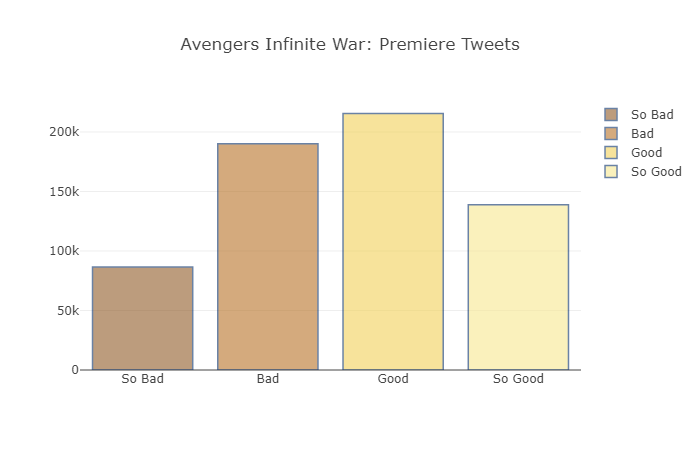
\includegraphics[width=5cm]{img/avengers.png} }}%
%     \qquad
%     \subfloat[Aquaman]{{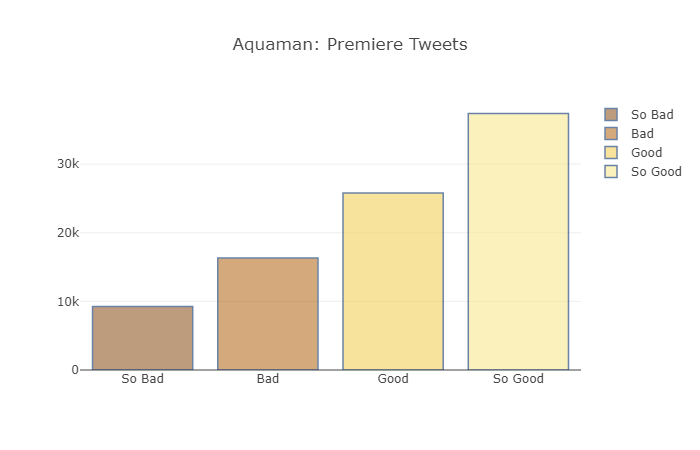
\includegraphics[width=5cm]{img/aquaman.png} }}%
%     \qquad
%     \subfloat[Captain Marvel]{{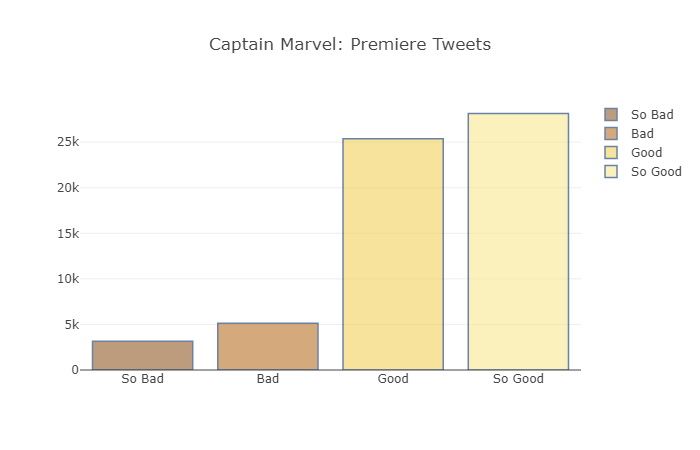
\includegraphics[width=5cm]{img/captain.png} }}%
%     \caption{Sentiment Analysis results on the tweets of each movie.}%
%     \label{fig:example}%
%     \end{center}
% \end{figure*}

%SO: esta subsection não seria dentro da B?
% I: SO, coloquei o mesmo comentário acima... Poderiam tirar esta divisão de seção e começar dizendo que neste trabalho foi usado o Vader, e, então, explicar o Vader.
%Ver vitor text ou words
Vader (Valence Aware Dictionary and sEntiment Reasoner)\footnote{https://github.com/cjhutto/vaderSentiment}
Lexicon is a lexicon based on sentiment-related words. In this approach, each word is labeled according to their semantic orientation as either positive or negative. Vader produces 4 sentiments metrics: the first three (positive, negative and neutral) represent the proportion of the words that match the categories. The final metric, \textit{compound} score, is a combination of the first three metrics normalized.
%SO normalizadas como?
The compound score ranges between -1 and 1, where -1 represents highly negative opinion and 1 highly positive opinion.

%Vader (Valence Aware Dictionary and sEntiment Reasoner) Lexicon is based on lexicon of sentiment-related words. In this approach, each words in the context are generally labeled according to their semantic orientation as either positive or negative. Vader produces 4 sentiments metrics: the first three, positive, negative and neutral, represent the proportion of the texts that matching into ant categories. The final metric, \textit{compound} score, is the sum of first three normalized metrics, between -1 and 1, that -1 represents highly negative and 1 highly positive.

%JS review
Since Vader deals with certain features that most of  other lexicon do not (such as Abbreviations, Upper Case, Emojis, and Special characters), it is considered a very appropriate lexicon to be used in Social Media texts evaluation. 
%SO: ref aqui... consderado por quem?
In the following example, we demonstrate the advantages of using Vader lexicon in Social Media.
% I: o exemplo mencionado acima é o da figura? Se sim, tem que colocar algo como "Through the example shown in Figure XXX".  

%We consider using Vader Lexicon, to evaluate the tweets texts, for supporting the following aspects that non-normalized text may contain: Abbreviations, Upper Case, Emojis, Special characters. To understand, how Vader is great alternative to text analysis, follow a example: 

\begin{figure}[htb]
    \begin{center}
        
\includegraphics[width=0.8\linewidth]{img/Twitter1.png}
    \end{center}
       \caption{Example of a tweet post} %using Vader Lexicon.}
    \label{fig:tweet1}
\end{figure}

% I: acho que "tweet" já apareceu antes e não estava em itálico. Acho que não precisa colocar Tweet e Twitter em itálico. Revisar isso em todo o paper.
The tweet presented in Figure~\ref{fig:tweet1} was evaluated with the following scores for sentiment analysis: \textit{'compound'}: 0.6133, \textit{'neg'}: 0.169, \textit{'neu'}: 0.508, \textit{'pos'}: 0.322. As we can see, the overall evaluation of the text denotes a positive emotion. But if this same text was parsed without considering \textit{emojis} and the emotional indication represented by capital letters, 
%SO: mudei um pouco a frase acima para explicar o "capital letters".. mas na verdade não entendi esse parágrafo, fiquei com muitas duvidas. Joana, podes passar aqui?
the scores evaluation would be: \textit{'compound'}: 0.2043, \textit{'neg'}: 0.202, \textit{'neu'}: 0.546, \textit{'pos'}: 0.251. In this case, we can notice a significant drop on the \textit{compound} value, which makes the text's emotion tending to neutral, instead of positive.% as it should.
%SO: tens que explicar o que são esses parametros? compound indica o que?

%The \textit{tweet} shown on Figure \ref{fig:tweet1} presented the following values for the sentiment analysis, \textit{'compound'}: 0.6133, \textit{'neg'}: 0.169, \textit{'neu'}: 0.508, \textit{'pos'}: 0.322, denoting a general positive evaluation (\textit{'compound'}: 0.6133). If the \textit{tweet} was parsed without \textit{emojis} and capital letters were not taken, the values obtained in the evaluation would be: \textit{'compound'}: 0.2043, \textit{'neg'}: 0.202, \textit{'neu'}: 0.546, \textit{'pos'}: 0.251. As we can see, the general evaluation of \textit{tweet} (\textit{compound}) dropped to 0,2043, which, although still a positive value, is closer to the neutral than previously obtained. 


\subsection{TF-IDF\label{TFID}}
%SO: esta sectionj não deveria estar dentro da B tb, como a section c?

\textit{Term Frequency-Inverse Document Frequency} indicates the weight of text's terms according to its frequency proportion~\cite{Dipanjan:2016} across documents. This %technique was developed to be a 
is a well-known metric in information retrieval. %classification metric for searching users' queries results on search engines.

%Term Frequency-Inverse Document Frequency, which indicates the weighting of terms occurring in texts, in proportion your frequency \cite{Dipanjan:2016}. This technique was developed as classification metric, in search results in search engines, based on user queries. 

% Isabel: é preciso explicar que fórmula é essa, para que serve.
%SO: mesmo comentário acima
\begin{equation*}
    W_{t,d} = \left ( \frac{Freq_{t,d}}{Max} \right ) * log_2 \left ( \frac{N}{n_t} \right),
\end{equation*}
where \( W_{t,d}\) represents the term weight \textit{t} in document \textit{d}. 
%SO: não entendi t é termo ou peso (weight?)
\( Freq_{t,d}\) is the number of times that the terms/words ($t$) occur in document \textit{d}. 
%SO: termo e work é a mesma coisa? então seria bom conceituar na primeira vez que aparece
\( Max\) is the term with the highest number of occurrences in the text. 
%SO: Max é o número máximo e não o termo que aparece certo? se sim, corrigir o texto acima...
%JS Rever!!! Vitor
\( N \) is the total of texts in the base of tests, \( n_t \) is the number of texts in the base of tests that owns the term \( t \). 



\subsection{Terms used for the characters}
% I: acho que heat map não precisa estar com letras maiúsculas. Abaixo seria: ...a visualization heat map... Revisar e padronizar em todo o texto. Estou achando estranho o início desta seção... Parece que vocês querem explicar como fazer heat map, mas na verdade é uma explicação sobre a contagem de ocorrência de termos por personagem, certo? Se for isso, tem que alterar até o título desta subseção. A motivação não é criar o heat map, a motivação é saber o que estão falando dos personagens, e o heat map é a maneira de visualizar isso. Sugestão para o título da seção: Terms used for the characters. Depois reescrever o início desta seção.
To understand how the public reacted to each character, it's necessary to have knowledge about the occurrences of the most used terms in relation to the main characters of a movie. This process is composed of 4 phases, as shown in Figure~\ref{fig:phases}. 
% I: alterei um pouco acima.

% I: tentei alterar o parágrafo abaixo, mas não entendi o que está sendo feito... Primeiro, vocês geram uma lista de personagens. Depois, o que é feito para cada personagem da lista? O que é gerado anteriormente? Estou pensando se a subseção de metodologia não deveria estar no início desta seção... A segunda frase abaixo eu acho que deveria começar por "Then, for each character from the list, we search...".
The first phase consists of collecting the list of main characters for a movie. Then, we search for each character in the list, in the set of already classified texts, and store the texts that have this condition in a temporary list. The third phase, we try to find in the resulting TF-IDF files, the terms classified as \textit{Adjectives} and that have at least 100 appearances in texts, and we also save in a temporary list. The last phase, is concerned with run the temporary list of text generated in phase 2, in the search for terms established in the phase 3. If condition is true, we add in a incremental variable, the number of times a given term is mentioned for each character. 

\begin{figure*}[btp]
\begin{center}
% \fbox{\rule{0pt}{2in} \rule{.9\linewidth}{0pt}}
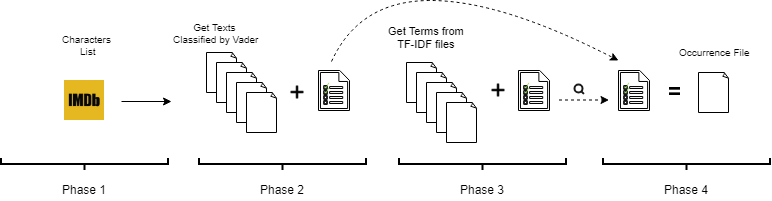
\includegraphics[width=0.8\linewidth]{img/diagrama-ocorrencia-movie.png}
\end{center}
   \caption{Occurrence Terms Model.}
\label{fig:phases}
\end{figure*}

% \subsection{Methodology}

\subsection{Data Analysis}

\textbf{Text Mining}

blablablabalbalblabalbalbblablablabalbalblabalbalbblablablaba lbalblabal balbblablablabalbal blabalbalbblablablab albalblabalbalbblablablabalbalblaba l balbbl abl ablaba lbalblabalbalbblablablabalbalblabalbalbblablablabalbalblabalbalbbla blablabalbalblabalbalbblablablabalbalblabalbalbblablablabalbalblabalbalbblablablabalbalblabalbalbblablablabalbalblabalbalb

\textbf{Sentiment Analysis}

blablablabalbalblabalbalbblablablabalbalblabalbalbblablablaba lbalblabal balbblablablabalbal blabalbalbblablablab albalblabalbalbblablablabalbalblaba l balbbl abl ablaba lbalblabalbalbblablablabalbalblabalbalbblablablabalbalblabalbalbbla blablabalbalblabalbalbblablablabalbalblabalbalbblablablabalbalblabalbalbblablablabalbalblabalbalbblablablabalbalblabalbalb

\textbf{Visualization}

In this step, we also generate 3 kinds of visualization graphics one for each social media we chose. The first one is a bar chart that displays the overall number of comments obtained for the selected movies on both social media. Each bar presented on this visualization represents one sentiment polarity (very positive, positive, negative and very negative). We opted to display the social media side by side to simplify users' comparison. 

The second visualization provides word clouds, showing the most used words for negative and positive sentiment polarity. For this visualization, we chose to use only verbs, noun, and adjective grammar types, because, for this case, we believe that those are the most significant ones. Like the previous visualization, 2 word clouds are generated for each social media, one for the most used words in negative comments, and another one for the most used words in positive comments. 

On the third visualization, a heatmap is presented. This visualization presents the top 10 most used adjectives in comments for the movie's characters. For this visualization, we present only characters for whom we were able to find mentions in the analyzed text. This visualization is split by sentiment polarity (positive and negative) and by social media (Twitter and YouTube). These visualizations can be seen in Figures ~\ref{fig:TotalOfInteractions},~\ref{fig:wordcloudsAquaman},~\ref{fig:wordcloudsCaptain},~\ref{fig:wordcloudsAvengers},~\ref{fig:AquamanCapitaHeatMap} and \ref{fig:VingadoresHeatMap}

\subsection{Text Recomendation}

%To establishing a textual standard, through Pos-Tag (Part-of-Speach) feature, we find for the terms classified as adjectives, within the results from most frequency terms, thus allowing the texts recommendation creation to each movie. 
%SO: lembrar que na introdução dissemos que geramos um meta texto de recomendação. Onde está isto no paper???

% Isabel: lembrar que nas seções abaixo é para descrever o que foi feito, algoritmos e visualizações. Mas, a análise dos filmes deve estar na próxima seção.



